
\subsection{Comparando Arquitecturas}

Ahora que se conoce el estado actual del sistema, al igual que estado de referencia; lo siguiente a realizar era la comparación de las arquitecturas. El resultado de esta, daría la base para poder decidir el qué hacer para adaptar el sistema y el cómo hacerlo.

Es necesario definir el como se realizará la evaluación del sistema. Esto no es tan sencillo como hacer una comparación usando un igual (\texttt{A == B}), ya que, el realizar esto, no resultaría realmente información sobre, qué, internamente, presenta problemas.

Ahora, la propiedades implementadas, definidas en los estados objetivo; son la manera las características principales por las cuales es posible realizar la evaluación del sistema. \textit{Timeout}, cumpliendo la función de establecer el tiempo máximo entre los reportes de dispositivos, definiendo cuando estos pueden considerarse como "vencidos"; y \textit{count}, como la cantidad de dispositivos en estado \textit{Coherent} mínima para el desarrollo de la aplicación.

Siendo así, se definió un proceso de comparación consta de evaluar cada componente del sistema en función de las propiedades. A partir de estas, es posible el evaluar el estado de la aplicación. Este proceso es descrito por la figura \ref{fig:LookerProcessClock}.

\begin{figure}[ht]
    \centering
    \caption{Proceso reloj realizado por el observador para la actualización del estado de la aplicación} 
    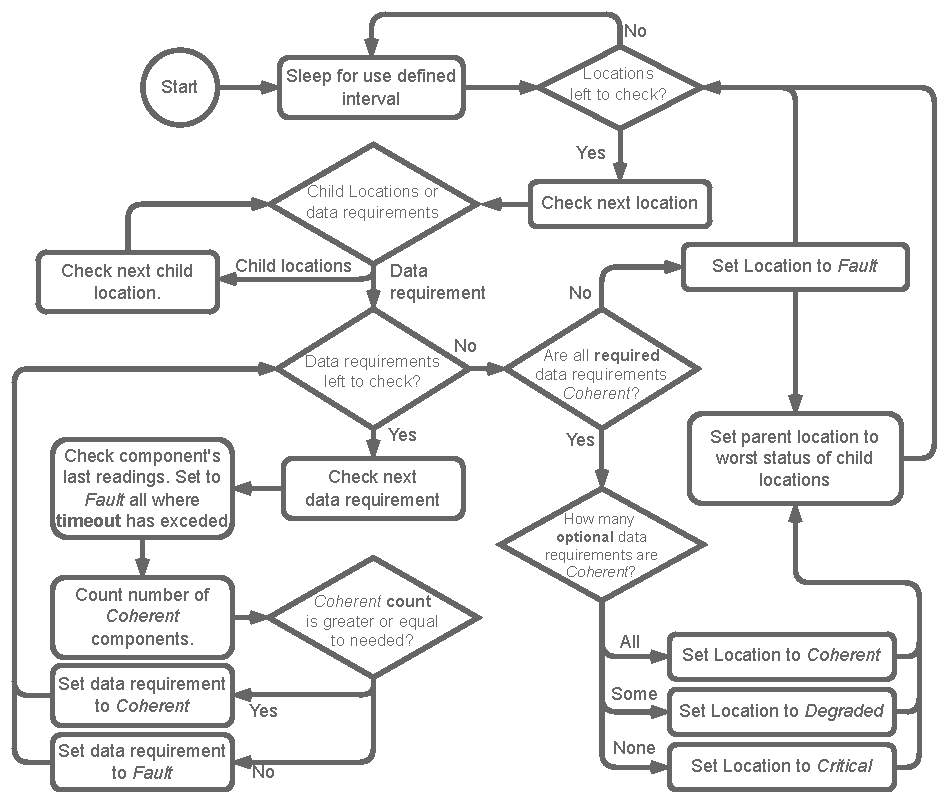
\includegraphics[width=0.85\linewidth]{images/LookerProcessClock.pdf}
    \label{fig:LookerProcessClock}
\end{figure} 

El proceso, apodado reloj, debido a su ejecución dado un intervalo de tiempo definido por el usuario; realiza la evaluación de la aplicación, recorriendo la estructura locación por locación. Siendo así, y con el fin de evitar una dispersión grande de los lugares de procesamiento, se implementó en \textit{Looker}.

Los componentes, pueden existir únicamente en un estado binario, sea \textit{Coherent}, en el caso de que cumplan con las condiciones establecidas en el requerimiento; o \textit{Fault} de lo contrario. Estos se basan únicamente en la propiedad \textit{timeout}, marcándolos de manera correspondiente a partir de su último reporte registrado. 

Así mismo, los requerimientos de datos, con la misma característica de su estado binario; usan propiedad \textit{count} para definir su condición. En caso de que la cantidad total de componentes sea igual a la requerida, se marcará como \textit{Coherent}; de lo contrario, estará en \textit{Fault}. Se ha de resaltar que, debido a que estas propiedades son opcionales durante la declaración, podrán presentarse casos en los que, dada una configuración específica, con un único reporte (o incluso ninguno) estos podrán considerarse válidos durante todo el de ejecución de la aplicación.

Una vez evaluadas los componentes y los requerimientos de datos, lo siguiente es evaluar la locación. Esto dependerá del tipo de la locación. Si es un agrupador, su estado será el peor de los estados de las hijas. De lo contrario, si tiene requerimientos de datos, su estado depende de sus requerimientos de datos y del tipo de cada uno de ellos.

El estado de estas locaciones se determina en dos pasos. En el primer paso, se verifica si alguno de sus requerimientos obligatorios está en estado \textit{Fault}. En ese caso, la locación se considera en estado \textit{Fault}, ya que no puede cumplir con los requisitos mínimos de la aplicación. Para las locaciones sin requerimientos opcionales, este será el final del proceso.

El segundo paso, en el caso de locaciones con requerimientos opcionales, el factor determinante será la cantidad de estados \textit{Coherent}. La locación tendrá un estado \textit{Critical}, \textit{Degraded}, o \textit{Coherent} según si todos, algunos o ninguno de estos requerimientos está en estado \textit{Fault}, respectivamente.

Esta manera de evaluar las locaciones permite el tener una idea más clara del estado de cada una de las locaciones, y por consiguiente, el estado de la aplicación. A partir de esta evaluación, se realizarán las diferentes adaptaciones necesarias con el fin de acercar el estado de la aplicación al estado de referencia esperado.

Una vez actualizado, y evaluado el estado; se tendría que reportar al agregador el nuevo estado de la aplicación. Para esto, se agregó un paso final tras la ejecución del proceso reloj, en la cual, \textit{Looker}, realiza una petición tipo \texttt{PUT} al endpoint designado en \texttt{Bran}, con el fin de actualizar el registro. La arquitectura del proyecto, hasta el momento, se puede ver en la figura \ref{fig:StarDuckBasic}.

\begin{figure}[ht]
    \centering
    \caption{Arquitectura actual del proyecto}
    \label{fig:StarDuckBasic}
    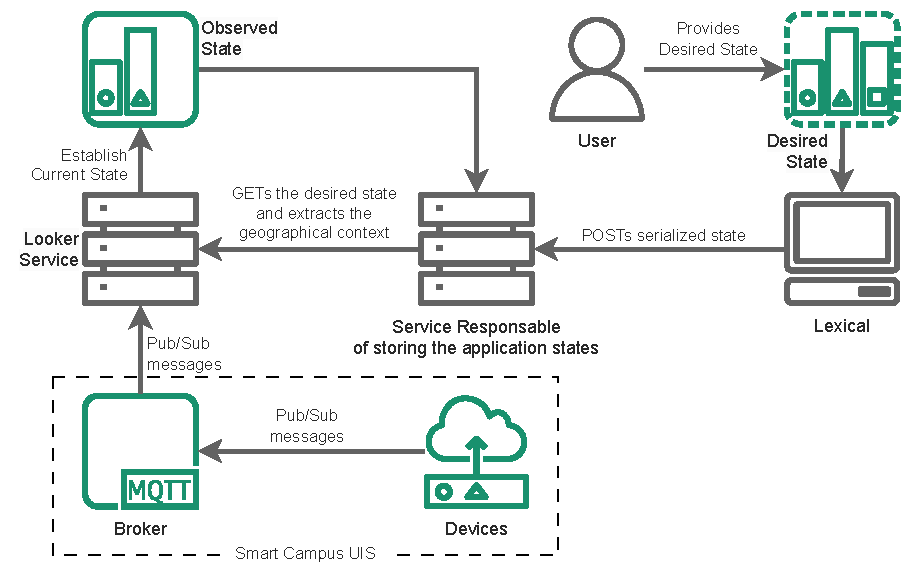
\includegraphics[width=0.8\linewidth]{images/StarDuckBasic.pdf}
\end{figure}


